\documentclass[11pt,a4paper]{article}
\usepackage{url}
\usepackage{graphicx}
\usepackage{makeidx}
\usepackage{amssymb}
\newcommand{\Butterfly}{\mbox{\large $\rhd\!\!\!\lhd$}}
\newcommand{\sync}[1]{\raisebox{-1.0ex}{$\;\stackrel{\Butterfly}{\scriptscriptstyle #1}\,$}}
\newcommand{\BioPEPA}{Bio-PEPA}
\newcommand{\BPWB}{{\BioPEPA} Workbench}
\newcommand{\StandardML}{Standard ML}
\newcommand{\MLton}{MLton}
\newcommand{\UNIX}{UNIX}
\newcommand{\ASCII}{ASCII}
\newcommand{\twinkle}{\begin{center}$\star$\end{center}}

\newcommand{\setting}[2]{\texttt{#1.#2}\index{Setting!#1!#2}}

\usepackage{latexsym}
\usepackage{alltt}
\usepackage{verbatim}
\usepackage{listings}

\makeindex
\begin{document}
\sloppy
\title{\bf The \BPWB:\\ User's Manual}
\author{Stephen Gilmore\\
  The University of Edinburgh}
\date{\today}
\maketitle
\tableofcontents

\section{Introduction}
This document describes the \BioPEPA\ Workbench version
     1.0 ``Charlie Mingus''%
, a tool for assisting with the analysis of systems
which are modelled in the \BioPEPA\ process algebra.  The definitive
reference for \BioPEPA\ is the technical report ``Bio-PEPA: a
framework for the modelling and analysis of biological systems'' by
Federica Ciocchetta and Jane Hillston\footnote{Available from
  \url{http://www.inf.ed.ac.uk/publications/report/1231.html}}.

The \BPWB\ and accompanying documentation such as this document can
be obtained via the World-Wide Web from the address
\url{http://homepages.inf.ed.ac.uk/stg/software/biopepa/}.

Given a Bio-PEPA model the Workbench generates a simulation model, a
Markov chain model and a differential equation model.  Thus the tool
enables the modeller to switch between discrete-state analysis via
simulation and model-checking and continuous-space analysis via
differential equations while maintaining only a single source model in
the Bio-PEPA language.

The \BPWB\ is intended for use with the stochastic simulation toolkit
``StochKit'', which features an implementation of the well-known
stochastic simulation algorithm (SSA) of Gillespie.
When given a Bio-PEPA model the \BPWB\ automatically generates other
representations in forms suitable for simulation and model-checking.
The generated simulation model contains the stoichiometry matrix and
propensity functions in the form of C++ code which is linked against
the StochKit simulation library for simulation with
Gillespie's Direct Method. 

The \BPWB\ generates the differential equation model in terms of a
high-level ``vector field'' representation used by the VFgen software
tool to generate ODE models suitable for analysis with the Sundials
ODE suite, Matlab, or many other tools.

The representation which is used for discrete state-space generation
and analysis by numerical solution of the underlying CTMC is expressed
in the reactive modules language supported by the PRISM model-checker.
PRISM provides algorithms for steady-state and transient analysis of
continuous-time Markov chains and model-checking of logical formulae
against CTMCs.  In addition the \BPWB\ generates reward structures and
common CSL formulae used in model-checking.

\section{Example 1: Simple Michaelis-Menten kinetics}
We describe the components of the \BioPEPA\ input language for the
Workbench via a simple example.  Consider Michaelis-Menten kinetics:
%%%%%%%%%%%%%%%%%%%%%%%%%%%%%%%%%%%%%%%%%%%%%%%%%%%%%%%%%%%%%%%%%%%%%%%%
\newcommand{\forcescriptsize}[1]{\hbox{\scriptsize\ensuremath{#1}}}%
\newcommand{\stackthree}[3]{\begin{array}{c}
    \forcescriptsize{#1}\\[-3pt] #2\\[-5pt] \forcescriptsize{#3}
    \end{array}}
\newcommand{\stacktwo}[2]{\stackthree{#1}{#2}{\phantom{#1}}}
%%%%%%%%%%%%%%%%%%%%%%%%%%%%%%%%%%%%%%%%%%%%%%%%%%%%%%%%%%%%%%%%%%%%%%%%
\begin{displaymath}
E + S \stackthree{k_1}{\rightleftharpoons}{k_{-1}} \textit{E:S}
      \stacktwo{k_2}{\rightarrow} E + P
\end{displaymath}
where an enzyme $E$ combines with a substrate $S$ to form a compound
\textit{E:S}.  This compound might degrade releasing the enzyme and
the substrate or it might convert the substrate into product $P$,
releasing the enzyme.

\subsection{A \BioPEPA\ model}
We could encode this model in \BioPEPA\ as shown below.



\begin{eqnarray*}
r_1 & = & [ k_1 \times  E \times  S ]\\%
r_{-1} & = & [ k_{-1} \times  \hbox{\textit{E:S}} ]\\%
r_2 & = & [ k_2 \times  \hbox{\textit{E:S}} ]\\%
%
E & = & r_1{\downarrow} +  r_{-1}{\uparrow}  +  r_2{\uparrow} \\%
S & = & r_1{\downarrow}  +  r_{-1}{\uparrow} \\%
\hbox{\textit{E:S}} & = & r_1{\uparrow}  +  r_{-1}{\downarrow}  +  r_2{\downarrow} \\%
P & = & r_2{\uparrow} \\%
%
(E \sync{\{r_1, r_{-1}, r_2\}} (S \sync{\{r_1, r_{-1}\}} (\hbox{\textit{E:S}} \sync{\{r_2\}} P)))%
\end{eqnarray*}
 
We have made use of aspects of the mathematical syntax for \BioPEPA\
in this definition.  Before simulating this model we first need to
encode it in the syntax accepted by the Workbench.  We place
these definitions in the file {\tt mm.biopepa}. 
This is a plain text file which can be edited using a text editor such
as TextPad or Emacs.  That file is shown in Figure~\ref{fig:mm.biopepa}.

\begin{figure}[htbp]
\verbatiminput{mm.biopepa}
\caption{\label{fig:mm.biopepa} The \texttt{mm.biopepa} file}
\end{figure}

In order to help with understanding the Bio-PEPA model the \BPWB\
generates a visualisation of the model in the form of a reaction
network graph where the species are represented as circles and the
reactions are represented using boxes.  This is a directed graph where
an arc leads from a species to a reaction if that species is a
reactant consumed by the reaction.  An arc leads in the other
direction (from a reaction to a species) if that species is a product
formed by the reaction.  An example of such a network is shown in
Figure~\ref{fig:mm.pdf}. 

\begin{figure}[htbp]
\begin{center}
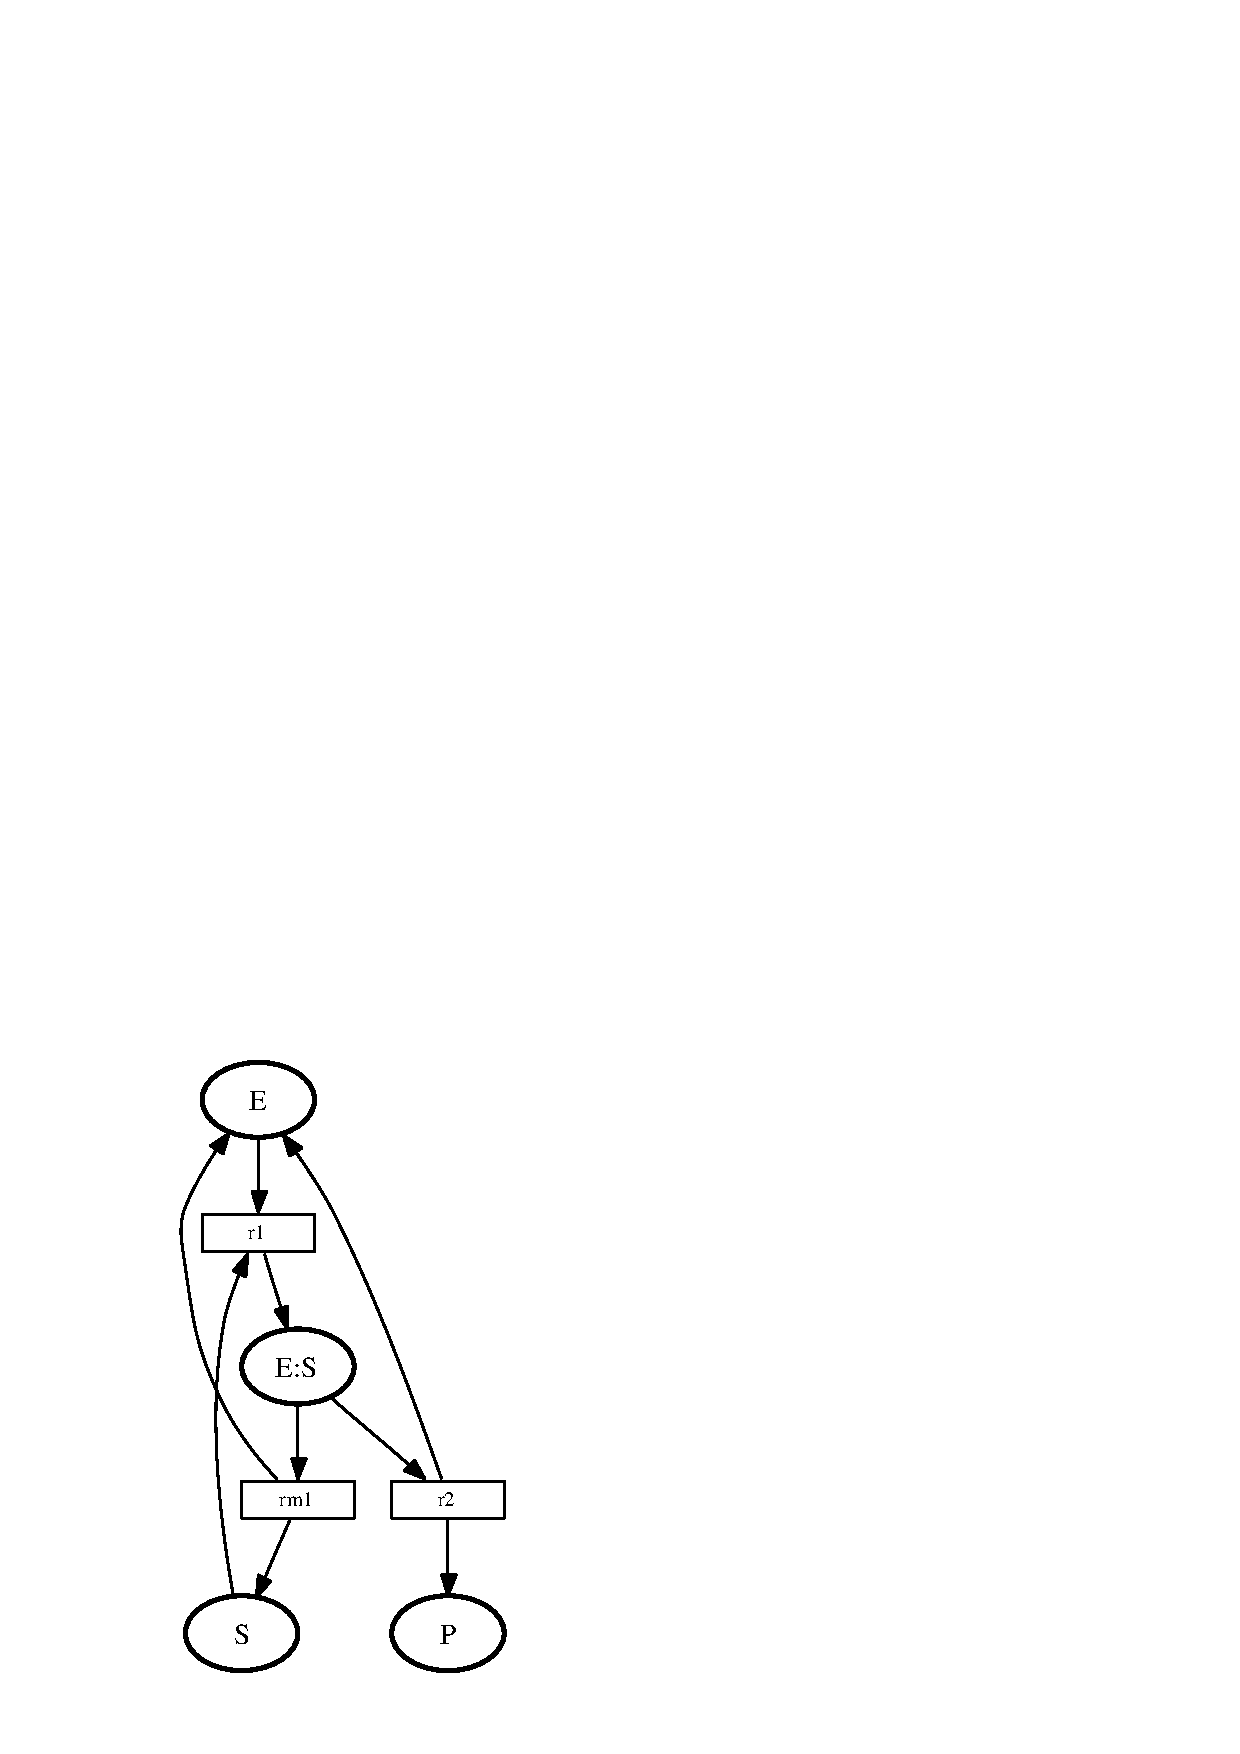
\includegraphics[scale=0.4]{mm.pdf}
\end{center}
\caption{\label{fig:mm.pdf} The reaction network graph generated 
  from the \texttt{mm.biopepa} file}
\end{figure}

\subsection{Parameter information}

Before we can simulate the model we require parameter data in the form
of the initial molecular counts of the four species involved ($E$,
$S$, \textit{E:S} and $P$) and the three rate constants ($k_1$,
$k_{-1}$ and $k_2$).  These should be stored in a comma-separated
value file named \texttt{mm.csv}.  That file is shown in 
Figure~\ref{fig:mm.csv}.

\begin{figure}[htbp]
\verbatiminput{mm.csv}
\caption{\label{fig:mm.csv} The \texttt{mm.csv} file}
\end{figure}

Space characters in the file are not significant and are only included
for readability above.  Comma-separated value files are also text
files and can be edited using text editors such as TextPad or Emacs
but they can also be conveniently edited using spreadsheet
applications such as Microsoft Excel or OpenOffice \texttt{oocalc}.


\section{Example 2: Michaelis-Menten with synthesis}

We will now consider a slightly more complex example which illustrates
other features of the Bio-PEPA language.  We will consider an example of
Michaelis-Menten with synthesis.

\subsection{The Bio-PEPA model}
\input{mms_biopepa} 


\subsection{Plotting with model components}

Occasionally it is convenient to have a series plotted which is a
function of some other series computed during the simulation.  It
would be possible to instrument a Bio-PEPA model with other species
whose purpose was just to generate these series but this would clutter
the model.  \emph{Model components} allow us to do this without
cluttering the model.  Consider \texttt{X} below.
\begin{verbatim}
X = [ A + B ];
\end{verbatim}
\texttt{X} is a model component whose function is to compute the
numerical sum of the value of \texttt{A} and \texttt{B} (where
\texttt{A} and \texttt{B} are species defined in Bio-PEPA in the usual
way).  Model component \texttt{X} should not participate in any
reactions and any initial value supplied for \texttt{X} in the
parameter file will be ignored (because its value is computed as the
sum of \texttt{A} and \texttt{B}).  Such a model component is used in 
our example of Michaelis-Menten with synthesis to track the total number
of molecules in the system.  This is \emph{not} a constant for this 
example because molecules can be synthesised from an outside source.


\section{Installing the \BPWB}

\newcommand{\ahref}[2]{#2\footnote{\url{#1}}}
\input{download}

\section{Running the \BPWB}

The \BPWB\ can be run by issuing the command \texttt{./bp} to compile
the input Bio-PEPA model, include the parameters from the model
parameter file and generate a report.  The output from the command
should be similar to the output shown in Figure~\ref{fig:bp.log}.
\begin{figure}[tbp]
\verbatiminput{bp.log}
\caption{\label{fig:bp.log} The output from the \BPWB}
\end{figure}

\section{Configuring the \BPWB}

The behaviour of the \BPWB\ can be configured by editing a
configuration file, \texttt{biopepa.cfg}.  The current version
of this file is shown in Figure~\ref{fig:biopepa.cfg}.
\begin{figure}[tbp]
\verbatiminput{cfg/biopepa.cfg}
\caption{\label{fig:biopepa.cfg} The \texttt{biopepa.cfg} configuration file}
\end{figure}

\subsection{Configuring simulations}

The simulator which is used to perform the simulation runs over the
generated simulation model is specified by the parameter
\setting{biopepa}{simulator}.  
%
The stop time of the simulation run is specified in the numerical
parameter value \setting{biopepa}{simulation.stoptime}.  Any
particular simulation run might terminate before this stop time is
reached if the reaction has run to completion already.
%
The defaults in the \texttt{biopepa.cfg} file are shown below.

\verbatiminput{cfg/biopepa.simulations.cfg}

\subsection{Configuring the number of replications}

The number of replications of the simulation which the \BPWB\ will
perform is controlled by the user-configurable numerical parameter
\setting{biopepa}{independent.replications}.
%
Whether all of the replications of the simulation are shown, or just  
the summary plot is controlled by the user-configurable Boolean parameter
\setting{biopepa}{show.all.replications}.
%
The defaults in the \texttt{biopepa.cfg} file are shown below.

\verbatiminput{cfg/biopepa.replications.cfg}


\subsection{StochKit options}

Detailed stochastic simulations give rise to files of data points
containing many thousands of points.  Writing out such large files is
slow and rendering them as graphs leads to large graphics files.  In
order to cut down the number of points reported, the user can set
\setting{stochkit}{opt.progress.interval}.  The default value is 1 but
any long-valued value may be used instead (e.g. \texttt{100},
\texttt{10000} or \texttt{1E10L}).
%
The default value in the \texttt{biopepa.cfg} file is shown below.

\verbatiminput{cfg/stochkit.opt.cfg}

\subsection{Reporting options}

While simulations are running it is often reassuring to receive a
report confirming that something is still happening.  However, if
doing many replications it is likely that one does not want to receive
a report for each one.  The integer-valued parameter
\setting{biopepa}{report.simulations.every} allows the user to choose
when they want to see these confirmation messages.
%
The parameter \setting{biopepa}{report.image.scale} scales the image
seen in the report written by the \BPWB.
%
The default values are shown below.

\verbatiminput{cfg/biopepa.report.cfg}


\section{Extending the \BPWB}

Some kinetic functions are predefined in \BioPEPA\@.  These include
the functions \texttt{fMA} (mass action kinetics), \texttt{fMM}
(Michaelis-Menten kinetics) and \texttt{fH} (Hill kinetics).  These
functions can be used in rate expressions but it might be convenient
to define other custom functions to be used in rate expressions in the
same way.  For this reason the \BPWB\ imports a file
\texttt{KineticFunctions.cpp} shown below.

\lstset{basicstyle=\tt\small,showstringspaces=false,stringstyle=\textit,commentstyle=\textit,keywordstyle=\textsl,language=C}%
\lstinputlisting[columns=flexible,basewidth={0.5em,0.4em}]{../../stochkit/test/BIOPEPA/DM/KineticFunctions.cpp}

This file implements the \texttt{fMA}, \texttt{fMM} and \texttt{fH}
functions but it can also be extended with other functions which are
convenient for other models.

\section{Report generation}

\subsection{Web page}

The \BPWB\ generates a Web page to allow users to preview their graphs
using a Web browser.  This presents a page of thumbnail images of the
graphs.  The graphs can be enlarged by clicking on them.  The enlarged
view can be repositioned in the browser by clicking and dragging.

\subsection{\LaTeX\ report}

The \BPWB\ generates a \LaTeX\ report with a formatted version of the
\BioPEPA\ model and the graphs generated from the simulation runs.

\section{Troubleshooting}

\subsection{``Command not found'' errors}

\begin{itemize}
\item I get a ``command not found'' error when trying to run the \BPWB.
      I typed \texttt{bp} but it gave me the following 
      error message: \texttt{bash: bp: command not found}.
      \begin{itemize}
      \item You need to tell Bash where to find the \texttt{bp}
         file.  If it is in the current working directory then the
         command which you should issue is \texttt{./bp}
      \end{itemize}
\end{itemize}

\subsection{``Permission denied'' errors}

\begin{itemize}
\item I get a ``permission denied'' error when trying to run the \BPWB.
      I typed \texttt{./bp} but it gave me the following 
      error message: \texttt{bash: ./bp: Permission denied}.
      \begin{itemize}
      \item You need to make the \texttt{bp} file executable.  Issue
            the command \texttt{chmod +x ./bp} and then try again.
      \end{itemize}
\end{itemize}


\subsection{``Cannot execute binary file'' errors}

\begin{itemize}
\item I get a ``cannot execute binary file'' error when trying to run the \BPWB.
      I typed \texttt{./bp} and the script started to run but it gave me the following 
      error message: \texttt{./bp: line 63: ./bin/biopepawb: cannot execute binary file}.
      \begin{itemize}
      \item You need to re-compile the \BPWB.  Issue
            the command \texttt{(cd src ; make)} and then try again.
      \end{itemize}
\end{itemize}

\subsection{``Cannot open'' errors}

\begin{itemize}
\item The \BPWB\ prints out a banner and then immediately says
      \texttt{Fatal error: Cannot open ``*.biopepa''}.
      \begin{itemize}
      \item You do not have a \BioPEPA\ file in the current 
            working directory.  Create a file using your favourite
            text editor and try again.  Remember to save the file 
            with the extension \texttt{.biopepa}
      \end{itemize}
\end{itemize}


\subsection{``Invalid parameter'' errors}

\begin{itemize}
\item The \BPWB\ seems to work and I even get some graphs but then it fails
      with the error 
      \texttt{Invalid Parameter - -thumbnail}.
      \begin{itemize}
      \item You need to download a newer version of the ImageMagick software
            and then try again.
      \end{itemize}
\end{itemize}


\subsection{``Undefined variable'' errors}

\begin{itemize}
\item The \BPWB\ seems to work up to the point of running the
  simulator but then it fails
      with the error 
      \texttt{undefined variable: bmargin}.
      \begin{itemize}
      \item You can either edit the \texttt{biopepa.cfg}
            file to change the value of 
            \texttt{gnuplot.key.position}
            or download a newer version of the 
            GnuPlot software
            and then try again.
      \end{itemize}
\end{itemize}

\printindex

\end{document}
\medskip


\newpage\noindent You now have three files which you did not have
before: {\tt tiny.table}, {\tt tiny.log} and {\tt
  tiny.maple}\footnote{The name of this file is instead {\tt tiny.m}
  for the Matlab version of the \BioPEPA\ Workbench.}.   These are text
files which can be read on the screen or searched using a \UNIX\ 
utility such as {\tt grep} or printed on a printer.  The real content
of the analysis is in {\tt tiny.maple} so we shall consider it first.  It
contains the entries for the transition matrix {\bf Q}.  Depicted
mathematically, {\bf Q} would be the matrix shown below where blank
entries indicate zeroes.  It does not matter for a tiny example such
as this one but as a general point the transition matricies of any
Markov processes are best stored within a computer as {\em sparse\/}
matricies.
\begin{center}
  \setlength{\arraycolsep}{0.5pt}
  $\left(\begin{array}{ccccccccc}
  -2 r_1 & r_1 & r_1 &  &  &  &  &  &  \\
    & -r_1 -r_2 &  & r_2 & r_1 & & & & \\
    &  &  -r_1 -r_2 & & r_1 & r_2 & & & \\
  r_3 & & & -r_1 -r_3 &  &  &  & r_1 & \\
     &   &   &   &  -2 r_2 &  & r_2 & r_2 & \\
  r_3 &  &  &  &  &  -r_1 - r_3 & r_1 & & \\
    &  r_3 &  &  &  &   & -r_2 - r_3 &  & r_2 \\
    &    &  r_3 &  &  &   &  &  -r_2 -r_3 & r_2 \\
    &  &  &  r_3 & & r_3  &   &  &  -2 r_3 \\
  \end{array}\right)$
\end{center}
The {\tt tiny.maple} file contains this matrix information in a
form suitable for consumption by a solution tool such as Matlab or
Maple.  When using the Matlab version of the Workbench the transitions
file would contain this.\par\medskip
\begin{small}
\begin{tt}\obeyspaces\obeylines
 \   Q(1,3) = Q(1,3) + r1;
 \   Q(1,1) = Q(1,1) - r1; \verb"%" \textit{t1 --start,r1-> t3}
 \   Q(1,2) = Q(1,2) + r1;
 \   Q(1,1) = Q(1,1) - r1; \verb"%" \textit{t1 --start,r1-> t2}
 \   ...
\end{tt}
\end{small}
\medskip\noindent
When using the Maple version of the Workbench the transitions
file would contain this.\par\medskip
\begin{small}
\begin{tt}\obeyspaces\obeylines
 \   Q[1,3] := Q[1,3] + r1:
 \   Q[1,1] := Q[1,1] - r1: \verb"#" \textit{t1 --start,r1-> t3}
 \   Q[1,2] := Q[1,2] + r1:
 \   Q[1,1] := Q[1,1] - r1: \verb"#" \textit{t1 --start,r1-> t2}
 \   ...
\end{tt}
\end{small}
\medskip\noindent [\textbf{Note:} The letter ``t'' is taken from the
first character of the filename (``tiny.pepa'' in this case).  If you wish to make
a detailed comparison of the state spaces generated by two separate
BioPEPA models then it is helpful to store them in files with different first
characters in the name (so that, for example, one state space is named
s1, s2, and s3 and the other is named t1, t2, and t3).]

\medskip\noindent The essence of the two presentations is the same.  A
square sparse matrix [the sparse element is zero] is modified by a
sequence of assignments which record the rate at which a transition
can move the system from one state to another.  Explanatory comments,
ignored by the solution package, give the identifier of the transition
and make clear the direction of the state change.  The comments are
stating this information: $3 \stackrel{a,r_1}{\longleftarrow} 1
\stackrel{a,r_1}{\longrightarrow} 2$.  This information is useful to
the modeller when examining the state space to detect symmetries
within the \BioPEPA\ model or when `debugging' a faulty model.
\twinkle
The states of the model have been associated with numbers for use as
the indices for the transition matrix.  Now we need to understand
which state has which number.  For this information we look at both
the files for the state table {\tt tiny.table} and (unless you specify
\texttt{-nohashing}) for the associated
hash table {\tt tiny.hash}.  These contain the information shown in
Figure~3.  The state table shows the assignment of state numbers to
states, identified in terms of their hash table identifier
equivalents.


\begin{figure}[htbp]
\begin{center}
  \begin{tabular}{cccc}
  {\bf The state table} 
&&&
  {\bf The hash table}\\
    $\begin{array}{rcl}
        1&\mapsto&a\parallel a\\
        2&\mapsto&d\parallel a\\
        3&\mapsto&a\parallel d\\
        4&\mapsto&g\parallel a\\
        5&\mapsto&d\parallel d\\
        6&\mapsto&a\parallel g\\
        7&\mapsto&d\parallel g\\
        8&\mapsto&g\parallel d\\
        9&\mapsto&g\parallel g\\
    \end{array}$
&&&
    $\begin{array}{rcl}
        P_1&\mapsto&a\\
        P_2&\mapsto&d\\
        P_3&\mapsto&g\\
        r_1&\mapsto&c\\
        r_2&\mapsto&f\\
        r_3&\mapsto&i\\
        \mathit{run}&\mapsto&e\\
        \mathit{start}&\mapsto&b\\
        \mathit{stop}&\mapsto&h\\
    \end{array}$
  \end{tabular}
\end{center}
\caption{State table and hash table for the tiny model.}
\end{figure}

Why have a state table?  The modeller using the Workbench needs to
know which states are which because certain states will be
distinguished success states or completion states or utilisation
states and the experimentation upon the model proceeds by considering
the effect on the model of changes of relative rate.

Why have a hash table?  All of the limiting problems with the use of
the \BioPEPA\ Workbench when processing large \BioPEPA\ models are to do
with space requirements either in terms of memory usage or disk usage.
In generating the state space of a model the Workbench may exhaust the
main memory capacity and fail.  In comparison the time taken to
process a model is of lesser importance because a modeller could
simply run the model for longer.  Thus when we attempt to improve the
\BioPEPA\ Workbench it is always by seeking to reduce the memory usage
[perhaps at the cost of some run-time penalty].  Problems related to
state-space size are a concern for all Markov modelling tools.

Notice that in the hash table no letters which were used as
identifiers in the \BioPEPA\ input are re-used as internal identifiers
within the Workbench.  This will not cause a difficulty if it happens 
but we take this opportunity to point out that---as with all model
development---the user should choose meaningful identifiers for the
activities, rates and components of a \BioPEPA\ model.
%%%
\twinkle At this point the \BioPEPA\ Workbench has done its work and it
is now time to use the available solution tool to solve the model to
find the steady state probability distribution.  Performance measures
can be calculated from this distribution.  For the particular
$9\times9$ matrix generated by the tiny example shown here it is as
easy to solve symbolically using Maple~(see Appendix~B) as it is to
solve numerically using Matlab~(see Appendix~A)\@.  For examples of
even moderate size seeking symbolic solutions becomes impractical.

\newpage
\noindent{\bf BioPEPA grammar}
\bigskip\newline\noindent
We now present the input grammar of the \ASCII\ syntax for the \BioPEPA\
language in {\small EBNF} notation.
\begin{displaymath}
\begin{array}{rcll}
  program      &::=& declaration^+ ~ \verb"(" ~ composition ~ \verb")"\\
  declaration  &::=& [\verb"#"] ~ id ~ \verb"=" ~ seq\_component ~ \verb";"\\
  seq\_component    
               &::=& seq\_component ~ \verb"/" ~ \verb"{" ~ [idseq] ~ \verb"}" 
               & \hbox{hiding}\\
               &\mid& seq\_component ~ \verb"+" ~ seq\_component 
               & \hbox{choice}\\
               &\mid& \verb"(" ~ id \verb"," ~ rate ~ \verb")"  ~
                      \verb"." ~ seq\_component 
               & \hbox{prefixing}\\
               &\mid& id 
               & \hbox{variable}\\
               &\mid& \verb"(" ~ seq\_component ~ \verb")" 
               & \hbox{grouping} \\
  composition  &::=& seq\_component ~ \verb"<" ~ [idseq] ~ \verb">" \\
               &   & \qquad 
                      seq\_component\\
               &\mid&  seq\_component ~ \verb"<" ~ [idseq] ~ \verb">"\\
               &   & \qquad 
                      composition\\ 
               &\mid& \verb"(" ~ composition ~ \verb")" \\
  idseq        &::=& id \\
               &\mid& id ~ \verb"," ~ idseq\\
  rate         &::=& id \\
               &\mid& int\\
               &\mid& \verb"infty" \\
  id           &::=& \hbox{alphanumeric sequence}\\
  int          &::=& \hbox{unsigned numeric sequence}
\end{array}
\end{displaymath}
In addition \LaTeX-style comments are supported, that is, the \BioPEPA\ 
Workbench ignores any characters which follow a percent sign on a
line.  Also, Java-style single-line comments are supported, beginning
with the sequence \verb"//".

The form of the component which follows the declaration sequence
should be a parallel composition of (a subset of) the components which
have been declared in the declaration sequence.  Note that parentheses
are mandatory around this component.

As noted above, a reserved word is used to represent the infinity
symbol which denotes that a component is passive with respect to this
action.  The reserved word is {\tt infty} [as in \TeX{} and \LaTeX]
where the symbol $\infty$ is used in the mathematical syntax for
\BioPEPA\@.

By convention, \BioPEPA\ components begin with an uppercase letter
whereas activity names begin with a lowercase letter.

\newpage
\paragraph{\bf Example sequential components:}

If {\tt P} and {\tt Q} are the only components declared in the
declaration sequence in the \BioPEPA\ program then the following are
legal component expressions which could appear in later declarations.
\newenvironment{examples}%%
  {\begin{center}\begin{tabular}{p{0.35\textwidth}p{0.55\textwidth}}}%%
  {\end{tabular}\end{center}}
\begin{examples}
  {\verb"P / {a}"}&Hiding any {\tt a} action of {\tt P}\\
  {\verb"P + Q"}&Choice between {\tt P} or {\tt Q}\\
  {\verb"(a, r1).P"}&Prefixing {\tt P} by {\tt a} with rate {\tt r1} \\
  {\verb"(a, 12).P"}&Prefixing {\tt P} by {\tt a} with rate 12 \\
  {\verb"(a, infty).P"}&Prefixing {\tt P} by {\tt a} performed passively\\
\end{examples}

\paragraph{\bf Sequential components non-examples:}

If {\tt P} and {\tt Q} are the only components declared in the
declaration sequence in the \BioPEPA\ program then the following are
illegal component expressions for the reason given.
\begin{examples}
  {\tt R}&Variable not declared\\
  {\verb"P \ {a}"}&The hiding symbol is the division sign\\
  {\verb"P / a"}&Set brackets are not optional\\
  {\verb"P <> Q"}&No use of parallel in sequential components \\
  {\verb"P.Q"}&No sequential composition in \BioPEPA \\
  {\verb"(a, r1) P"}&Omitted full stop \\
  {\verb"(a, 12.0).P"}&Real number constants not allowed \\
  {\verb"(a, 5 / 2).P"}&No arithmetic operations; only constants \\
  {\verb"P[b/a]"}&No renaming in \BioPEPA \\
\end{examples}

\paragraph{\bf Example parallel compositions:}

If {\tt P} and {\tt Q} are the only components declared in the
declaration sequence in the \BioPEPA\ program then the following are
legal parallel compositions which could appear after the 
declarations.
\begin{examples}
  {\verb"(P <> Q)"}&{\tt P} and {\tt Q} proceed independently in parallel\\
  {\verb"(P <a, b> Q)"}&{\tt P} and {\tt Q} synchronise on {\tt a} and
  {\tt b}\\
  {\verb"((P <> P) <a, b> (Q <> Q))"}&Copies of {\tt P} and {\tt Q} synchronise on {\tt a} and
  {\tt b}\\
\end{examples}

\paragraph{\bf Parallel compositions non-examples:}

If {\tt P} and {\tt Q} are the only components declared in the
declaration sequence in the \BioPEPA\ program then the following are
illegal parallel compositions for the reason given.
\begin{examples}
  {\tt P}&Composition not enclosed in parentheses\\
  {\tt (R)}&Variable not declared\\
  {\verb"(P | Q)"}&Pure parallel composition symbol is \verb"<>"\\
  {\verb"(P < a b > Q)"}&Omitted comma\\
  {\verb"((a, r1).P)"}&No sequential operations in the composition \\
\end{examples}


%%%%%%%%%%%%%%%%%%%%%%%%%%%%%%%%%%%%%%%%%%%%%%%%%%%%%%%%%%%%%%%%%%%%%%%%
%%%%%%%%%%%%%%%%%%%%%%%%%%%%%%%%%%%%%%%%%%%%%%%%%%%%%%%%%%%%%%%%%%%%%%%%
%%%%%%%%%%%%%%%%%%%%%%%%%%%%%%%%%%%%%%%%%%%%%%%%%%%%%%%%%%%%%%%%%%%%%%%%
%%%%%%%%%%%%%%%%%%%%%% BioPEPA NETS %%%%%%%%%%%%%%%%%%%%%%%%%%%%%%%%%%%%%%%
%%%%%%%%%%%%%%%%%%%%%%%%%%%%%%%%%%%%%%%%%%%%%%%%%%%%%%%%%%%%%%%%%%%%%%%%
%%%%%%%%%%%%%%%%%%%%%%%%%%%%%%%%%%%%%%%%%%%%%%%%%%%%%%%%%%%%%%%%%%%%%%%%
%%%%%%%%%%%%%%%%%%%%%%%%%%%%%%%%%%%%%%%%%%%%%%%%%%%%%%%%%%%%%%%%%%%%%%%%

\newpage
\noindent{\bf Modelling with \BioPEPANets}

\bigskip\noindent
The following input file describes a \BioPEPANet.  The model description
has several parts.  First, components as described just as they would
be in \BioPEPA\@.  Then places in the net are specified, including cells
which can contain a \BioPEPA\ component (circulating around the net).
The initial marking is specified at this stage.  Some places are
empty, but every place suggests the type of component which it should
contain.  (For example ``\texttt{Agent[\_]}'' denotes a currently
empty place, which could in the future contain an agent.)  Some cells
already have a \BioPEPA\ component in one of its local states
(``\texttt{Agent[Agent]}'' is an agent-type cell which contains an
agent in its initial state).  Arcs from place to place describe the
structure of the net.  Arcs are labelled with an activity name and a
rate.  For example, ``\texttt{P2 -(go, lambda)-> P3}'' denotes that
there is an arc from place \texttt{P2} to place \texttt{P3} which can
be crossed by a component which performs the \texttt{go} activity.
When the component performs that activity it will move from place
\texttt{P2} to place \texttt{P3} and experience any change of state
which it would experience through performing that activity.  (For
example, transitioning from the \texttt{Agent} state to the
\texttt{Agent1} state.)

\verbatiminput{mobileagent.pepa}


\newpage
\noindent{\bf Experimenting with a model}
\bigskip\newline\noindent
Finding the equilibrium probability distribution for a model is an
important first step in investigating its behaviour.  Once this has
been achieved the modeller can conduct a series of experiments to
investigate the model thoroughly.  The series of experiments
which are undertaken will vary from model to model but they commonly
involve selecting an interesting subset of the state space and finding
the probability of being in those states.  An activity which must be
performed in doing this part of the experimentation is finding the
numbers which are associated with the states which are of interest.
We provide another tool to assist with this: the tool is called the
\BioPEPA\ State Finder.

The modeller first describes some states of interest through the use
of a simple pattern language with stars for wild cards and vertical
bars for separators between model components.  Returning to our tiny
example, a modeller interested in testing how often either component
in the tiny example was component \texttt{P1} would prepare a file
called \texttt{tiny.psf} with the following contents.\par
\begin{small}
\begin{verbatim}
      % We are checking for P1 in either case
      test: P1|*
      test: *|P1
\end{verbatim}
\end{small}
The identifier \texttt{test} gives the name of the function and after
the colon comes the pattern of interest.  Assuming that you access the
\BioPEPA\ State Finder by typing {\tt psf} then the function is processed as
shown in Figure~3 where the user only typed the {\tt psf} command, the
model name and the function name and the rest was produced by the tool.
\begin{figure}[htbp]
\begin{small}
\begin{tt}\obeyspaces\obeylines
 \   [unix]: \textit{psf} 
 \   BioPEPA State Finder [Version \PSFversion, \textsl{solver}, \PSFcompiled]
 \   BioPEPA model name: \textit{tiny}
 \   PSF file name: \textit{tiny}
 \   Function ``test'' written to file ``test.fun''.
 \   Exiting BioPEPA State Finder.
\end{tt}
\end{small}
\caption{A sample \BioPEPA\ State Finder session}
\end{figure}

\noindent 
The function which was generated by this is shown in Appendix~C\@.  For
this tiny example the function could easily have been created by hand
since the model has a very regular structure and only nine states but
with larger models the usefulness of the \BioPEPA\ State Finder becomes
clearer.   Notice that here the tool correctly avoids counting the
state $P_1 \parallel P_1$ twice.  This would be a mistake which could
easily be made otherwise.

The \BioPEPA\ State Finder must be run after running the \BioPEPA\ Workbench
on a model because it searches through the table file which the
Workbench produces.  

\newpage
\noindent{\bf Limitations}
\bigskip\newline\noindent
\newcommand{\BUG}{This is an error which should be corrected in later
  versions of the \BioPEPA\ Workbench.}
The \BioPEPA\ Workbench has a number of limitations.
\begin{itemize}\setlength{\itemsep}{0pt}

\item The Workbench implements Cyclic \BioPEPA\ only (see [Hillston,
  1996] for the definition of this term).  These are the only \BioPEPA\ 
  models for which steady-state probability distributions can be
  calculated.  This is a consequence of the language definition and 
  will not be changed.

%%%Believed to be fixed in Version 0.62
%%%
%%%\item The Workbench does not implement the multigraph semantics of
%%%  \BioPEPA\ correctly.  This means that if a \BioPEPA\ component could
%%%  perform a particular action at the same rate and arrive at the same
%%%  resulting state in more than one way then it will not be
%%%  processed correctly.  A declaration such as the following will not
%%%  be interpreted as it should be according to the \BioPEPA\ semantics,
%%%  for any previously declared {\tt Q}.
%%%\begin{verbatim}
%%%#P = (a, r1).Q + (a, r1).Q;
%%%\end{verbatim}
%%%  \BUG\ A `workaround' for this error is for the user to calculate by
%%%  hand the equivalent effect and implement this.  Here the workaround
%%%  would be to write
%%%\begin{verbatim}
%%%#P = (a, twice_r1).Q;
%%%\end{verbatim}
%%%  where \verb"twice_r1" is a fresh identifier name which is to be
%%%  assigned a value which is twice that of \verb"r1".

\item The Workbench does not implement the apparent rates of \BioPEPA\@.
  All synchronisations must be between one active component and one
  passive component. \BUG

%%%Believed to be fixed in Version 0.72
%%%\item The Workbench does not do any semantic analysis of the program
%%%  before beginning to compute the state space.  This could mean that a
%%%  model would run for a very long time and then stop with the message
%%%\begin{verbatim}
%%%uncaught exception UndeclaredIdentifier
%%%\end{verbatim}

%%%\item The Workbench does not treat {\tt tau} as a reserved word and
%%%  will incorrectly allow components to synchronise on {\tt tau}
%%%  actions which appear in synchronisations.  \BUG

%%%\item The parser gives very poor error messages in some cases.  This
%%%  can mean that the person using the Workbench has to look through
%%%  their entire program to find the error.

%%%Don't be so modest!!
%%%\item The Workbench uses a lot of memory and runs quite slowly.
  
\end{itemize}

\newpage
\noindent{\bf Appendix A: \ A sample MATLAB session}
\bigskip\newline\noindent
In this appendix the nine state model is solved for the particular
case when $r_1=r_2=r_3=2.0$.  Since all of the transitions proceed at
the same rate, and the model is symmetric, all of the states are
equally likely, with calculated probability $\frac19\approx0.1111$.
\begin{alltt}
[unix]: \textit{matlab -nodesktop -nosplash -nojvm}

                      < M A T L A B >
            Copyright 1984-2005 The MathWorks, Inc.
            Version 7.0.4.352 (R14) Service Pack 2
                      January 29, 2005


  To get started, type one of these: helpwin, helpdesk, or demo.
  For product information, visit www.mathworks.com.
 
>> \textit{Q=sparse(9,9);}
>> \textit{r1=2.0;}
>> \textit{r2=2.0;}
>> \textit{r3=2.0;}
>> \textit{tiny;}
>> \textit{for i=1:9}
     \textit{Q(i,9) = 1.0;}
   \textit{end}
>> \textit{b=zeros(9,1);}
>> \textit{b(9) = 1.0;}
>> \textit{QT = Q';}
>> \textit{P = QT}\verb"\"\textit{b}

P =

    0.1111
    0.1111
    0.1111
    0.1111
    0.1111
    0.1111
    0.1111
    0.1111
    0.1111

>> \textit{quit}

\end{alltt}


\newpage
\noindent{\bf Appendix B: \ A sample Maple session}
\bigskip\newline\noindent
In this appendix the nine state model is solved symbolically for all
values of  $r_1$, $r_2$ and $r_3$.
\begin{alltt}
[unix]: \textit{maple}
{\small\verb"   |\^/|    "Maple 9 (IBM INTEL LINUX)}
{\small\verb"_|\|   |/|_ "Copyright (c) Maplesoft, a division of Waterloo Maple Inc. 2003}
{\small\verb"\  MAPLE  / "All rights reserved. Maple is a trademark of}
{\small\verb"<____ ____> "Waterloo Maple Inc.}
{\small\verb"     |      "Type ? for help.}
> \textit{with(linalg):}
Warning, the protected names norm and trace have been redefined and unprotected
> \textit{Q := array(sparse,1..9,1..9):}
> \textit{read `tiny.maple`:}
> \textit{b := array(sparse,1..9):}
> \textit{for i to 9 do}
  \textit{    Q[i,9] := 1.0}
  \textit{od:}
> \textit{b[9] := 1:}
> \textit{QT := transpose(Q):}
> \textit{P := linsolve(QT,b);}
\begin{small}
              2   2    2          2             2       2   2   
            r3  r2   r3  r2 r1  r3  r2 r1  r3 r2  r1  r3  r1   
     P := [ -------, ---------, ---------, ---------, -------, 
               %1        %1         %1         %1        %1    

              2             2          2    2   2
         r3 r2  r1  r3 r2 r1   r3 r2 r1   r1  r2
         ---------, ---------, ---------, ------- ]
             %1        %1         %1        %1

              2        2   2     2   2           2     
%1 := 2. r3 r2  r1 + r3  r2  + r1  r2  + 2. r2 r1  r3 +
                 2     2   2
      2. r2 r1 r3  + r3  r1
\end{small}
> \textit{quit}
bytes used=1962176, alloc=1638100, time=0.18
\end{alltt}

\newpage
\noindent{\bf Appendix C: \ A function generated by the BioPEPA state finder}
\bigskip\newline\noindent
This is the function which was generated when the \texttt{tiny.psf}
file was processed by the \BioPEPA\ State Finder.  The 
body of the \texttt{test} function adds together the
probabilities for the relevant states.   After a comment symbol on
each line comes the description of the state.  As we expected, all of
the states contain a $P_1$ component.
\bigskip\newline\noindent\par
\begin{small}
\begin{tt}\obeyspaces\obeylines
 \ \null
 \   \verb"#"  Function: test
 \   \verb"#"  Table:  \kern1ex tiny.table
 \ \null
 \   test := proc (P)
 \   (       0
 \           +  P[1] \verb"#" P1|P1
 \           +  P[3] \verb"#" P1|P2
 \           +  P[6] \verb"#" P1|P3
 \           +  P[2] \verb"#" P2|P1
 \           +  P[4] \verb"#" P3|P1
 \   )
 \   end:
 \ \null
 \   print (`BioPEPA: Defined function ``test'.  Usage: test(P);`);
\end{tt}
\end{small}


\newpage
\noindent{\bf Appendix D: \ Installing and running the \BPWB}
\bigskip\newline\noindent
The \BPWB\ is a \StandardML\ application.  It is available both in
source code form and as pre-compiled binaries for Linux and Windows.
We have tested the \BPWB\ on Linux Fedora Core~3 and Windows~XP, as
well as earlier versions of these operating systems.  The
\BioPEPAversion\ release of the \BPWB\ has been compiled using the
\MLton\ compiler for \StandardML, but can also be compiled using other
compilers for the language.  The \BPWB\ does not need root or
Administrator privileges to build and install, and the pre-compiled
binaries will run from the current working directory.  The Workbench
can reside in any directory on the filesystem and always writes files
to the directory in which the \BioPEPA\ (or \BioPEPANet) model resides.  The
compiled image of the Workbench is not large (about 1 Megabyte).
%
\bigskip\newline\noindent
\noindent{\bf D.1\ \ Running under Windows with Cygwin}
\medskip\newline\noindent
The compiled version of the \BPWB\ is stored in \texttt{pwb.exe}.  It
depends on the Cygwin implementation of \UNIX\ for Windows.  Before
installing the \BPWB\ you should first install Cygwin (from
\texttt{www.cygwin.com}).  We have tested the \BPWB\ with Cygwin
version 1.5.18-1.  The \BPWB\ depends on the dynamically-linked
library \texttt{cygwin1.dll}, and will not operate without it.

\BioPEPA\ and \BioPEPANet\ source files may be stored in any folder, even if
the folder contains spaces in the name as in the following example.
\begin{verbatim}
./pwb -nohashing C:/Documents\ and\ Settings/user/My\ Documents/tiny.pepa
\end{verbatim}
\medskip\noindent{\bf D.2\ \ Running under Linux}
\medskip\newline\noindent
The compiled version of the \BPWB\ is stored in \texttt{pwb}.  It
expects to access the C library \texttt{glibc} version 2.2.5 or
higher.  We have tested the compiled version with \texttt{glibc}
version 2.3.5. 
%
\bigskip\newline\noindent
\noindent{\bf D.3\ \ Building the \BPWB\ from source}
\medskip\newline\noindent
For other platforms for which a binary version of the \BPWB\ is not
provided first obtain an implementation of the \StandardML\
programming language and modify the Makefile in the source directory
to compile the Workbench using your chosen \StandardML\ compiler.
Re-compile the Workbench with \texttt{make mlton}.

\end{document}
